%%%%%%%%%%%%%%%%%%%%%%%%%%%%%%%%%%%%%%%%%
% Wenneker Assignment
% LaTeX Template
% Version 2.0 (12/1/2019)
%
% This template originates from:
% http://www.LaTeXTemplates.com
%
% Authors:
% Vel (vel@LaTeXTemplates.com)
% Frits Wenneker
%
% License:
% CC BY-NC-SA 3.0 (http://creativecommons.org/licenses/by-nc-sa/3.0/)
% 
%%%%%%%%%%%%%%%%%%%%%%%%%%%%%%%%%%%%%%%%%

%----------------------------------------------------------------------------------------
%	PACKAGES AND OTHER DOCUMENT CONFIGURATIONS
%----------------------------------------------------------------------------------------

\documentclass[11pt]{scrartcl} % Font size

%%%%%%%%%%%%%%%%%%%%%%%%%%%%%%%%%%%%%%%%%
% Wenneker Assignment
% Structure Specification File
% Version 2.0 (12/1/2019)
%
% This template originates from:
% http://www.LaTeXTemplates.com
%
% Authors:
% Vel (vel@LaTeXTemplates.com)
% Frits Wenneker
%
% License:
% CC BY-NC-SA 3.0 (http://creativecommons.org/licenses/by-nc-sa/3.0/)
% 
%%%%%%%%%%%%%%%%%%%%%%%%%%%%%%%%%%%%%%%%%

%----------------------------------------------------------------------------------------
%	PACKAGES AND OTHER DOCUMENT CONFIGURATIONS
%----------------------------------------------------------------------------------------

\usepackage{amsmath, amsfonts, amsthm} % Math packages

\usepackage{listings} % Code listings, with syntax highlighting

\usepackage{xcolor} % Color extensions

\usepackage{cleveref} % Smarter referencing to labels {figures, tables, etc...}
\crefname{lstlisting}{listing}{listings}
\Crefname{lstlisting}{Listing}{Listings}

\usepackage[english]{babel} % English language hyphenation

\usepackage{graphicx} % Required for inserting images
\graphicspath{{Figures/}{./}} % Specifies where to look for included images (trailing slash required)

\usepackage{booktabs} % Required for better horizontal rules in tables

\usepackage{parskip} % Automatically insert newline

\numberwithin{equation}{section} % Number equations within sections (i.e. 1.1, 1.2, 2.1, 2.2 instead of 1, 2, 3, 4)
\numberwithin{figure}{section} % Number figures within sections (i.e. 1.1, 1.2, 2.1, 2.2 instead of 1, 2, 3, 4)
\numberwithin{table}{section} % Number tables within sections (i.e. 1.1, 1.2, 2.1, 2.2 instead of 1, 2, 3, 4)

\setlength\parindent{0pt} % Removes all indentation from paragraphs

\usepackage{enumitem} % Required for list customisation
\setlist{noitemsep} % No spacing between list items

%----------------------------------------------------------------------------------------
%	DOCUMENT MARGINS
%----------------------------------------------------------------------------------------

\usepackage{geometry} % Required for adjusting page dimensions and margins

\geometry{
	paper=a4paper, % Paper size, change to letterpaper for US letter size
	top=2.5cm, % Top margin
	bottom=3cm, % Bottom margin
	left=3cm, % Left margin
	right=3cm, % Right margin
	headheight=0.75cm, % Header height
	footskip=1.5cm, % Space from the bottom margin to the baseline of the footer
	headsep=0.75cm, % Space from the top margin to the baseline of the header
	%showframe, % Uncomment to show how the type block is set on the page
}

%----------------------------------------------------------------------------------------
%   Listing Style	
%----------------------------------------------------------------------------------------

\definecolor{ao}{rgb}{0.0, 0.5, 0.0}

\lstdefinestyle{CStyle}{
  language=C,                     % choose the language of the code
  numbers=left,                   % where to put the line-numbers
  stepnumber=1,                   % the step between two line-numbers.        
  numbersep=5pt,                  % how far the line-numbers are from the code
  backgroundcolor=\color{white},  % choose the background color. You must add \usepackage{color}
  commentstyle=\color{ao},
  keywordstyle=\color{blue},
  showspaces=false,               % show spaces adding particular underscores
  showstringspaces=false,         % underline spaces within strings
  showtabs=false,                 % show tabs within strings adding particular underscores
  tabsize=2,                      % sets default tabsize to 2 spaces
  captionpos=b,                   % sets the caption-position to bottom
  breaklines=true,                % sets automatic line breaking
  breakatwhitespace=true,         % sets if automatic breaks should only happen at whitespace
  title=\lstname,                 % show the filename of files included with \lstinputlisting;
}

%----------------------------------------------------------------------------------------
%	FONTS
%----------------------------------------------------------------------------------------

\usepackage[utf8]{inputenc} % Required for inputting international characters
\usepackage[T1]{fontenc} % Use 8-bit encoding

\usepackage{fourier} % Use the Adobe Utopia font for the document

%----------------------------------------------------------------------------------------
%	SECTION TITLES
%----------------------------------------------------------------------------------------

\usepackage{sectsty} % Allows customising section commands

\renewcommand\thesubsection{\alph{subsection}} % Alpha subsection numbering 

\sectionfont{\vspace{6pt}\centering\normalfont\scshape} % \section{} styling
\subsectionfont{\normalfont\bfseries} % \subsection{} styling
\subsubsectionfont{\normalfont\itshape} % \subsubsection{} styling
\paragraphfont{\normalfont\scshape} % \paragraph{} styling

%----------------------------------------------------------------------------------------
%	HEADERS AND FOOTERS
%----------------------------------------------------------------------------------------

\usepackage{scrlayer-scrpage} % Required for customising headers and footers

\ohead*{} % Right header
\ihead*{} % Left header
\chead*{} % Centre header

\ofoot*{} % Right footer
\ifoot*{} % Left footer
\cfoot*{\pagemark} % Centre footer
 % Include the file specifying the document structure and custom commands

%----------------------------------------------------------------------------------------
%	TITLE SECTION
%----------------------------------------------------------------------------------------

\title{	
	\normalfont\normalsize
	\textsc{Curtin University, Concurrent Systems}\\ % Your university, school and/or department name(s)
	\vspace{25pt} % Whitespace
	\rule{\linewidth}{0.5pt}\\ % Thin top horizontal rule
	\vspace{20pt} % Whitespace
	{\huge Lab report 2}\\ % The assignment title
	\vspace{12pt} % Whitespace
	\rule{\linewidth}{2pt}\\ % Thick bottom horizontal rule
	\vspace{12pt} % Whitespace
}

\author{\LARGE Nhan Dao} % Your name

\date{\normalsize\today} % Today's date (\today) or a custom date

\begin{document}

\maketitle % Print the title

%----------------------------------------------------------------------------------------
%  Monte Carlo's extimation of Pi using POSIX's pthreads	
%----------------------------------------------------------------------------------------

\section{Monte Carlo's estimation of Pi using POSIX's pthreads}

\subsection{Briefly explain the difference between a process and a thread}

A process can have multiple threads, these threads are considered within the process by the kernel.
Being a part of the same process, threads shares instruction, global, and heap region of memory.

A multi-process program has memory space for each process, hence inter-process communication is slow
because memory is not shared between them unlike threads. Context switching between process is more
expensive compared to threads - which means when the OS/Kernel switch to executing a different processes,
it has to reload the registers to regain the context for that execution, this does not happen with threads.

%------------------------------------------------

\subsection{Creating \& Joining threads using POSIX}

\Cref{lst:lab2part1a} and \cref{lst:lab2part1b} shows the creation and joining of POSIX threads.

\vspace{0.5cm}
\lstinputlisting[
	style=CStyle,
	firstline=45, % First line of code
	lastline=48, % Lastl ine of code
	caption=Creating Pthreads (line 45-48 in lab2part1.c), % Caption above the listing
	label=lst:lab2part1a, % Label for referencing this listing
	frame=single, % Frame around the code listing
	showstringspaces=false, % Don't put marks in string spaces
	numbers=left, % Line numbers on left
	numberstyle=\normalsize % Line numbers styling
	]{../code/lab2part1.c}

\vspace{0.5cm}
\lstinputlisting[
	style=CStyle,
	firstline=49, % First line of code
	lastline=51, % Lastl ine of code
	caption=Joining Pthreads (line 49-51 in lab2part1.c), % Caption above the listing
	label=lst:lab2part1b, % Label for referencing this listing
	frame=single, % Frame around the code listing
	showstringspaces=false, % Don't put marks in string spaces
	numbers=left, % Line numbers on left
	numberstyle=\normalsize % Line numbers styling
	]{../code/lab2part1.c}

%------------------------------------------------

\subsection{Generating random uniformly distributed dart tosses}

\Cref{lst:lab2part1c} shows the subroutine that generates uniformly distributed dart tosses between [-1, 1].
Each worker thread runs this subroutine, and counts the number of tosses that falls within the unit circle.

\vspace{0.5cm}
\lstinputlisting[
	style=CStyle,
	firstline=82, % First line of code
	lastline=89, % Lastl ine of code
	caption=Generating uniformly distributed dart tosses (line 82-89 in lab2part1.c), % Caption above the listing
	label=lst:lab2part1c, % Label for referencing this listing
	frame=single, % Frame around the code listing
	showstringspaces=false, % Don't put marks in string spaces
	numbers=left, % Line numbers on left
	numberstyle=\normalsize % Line numbers styling
	]{../code/lab2part1.c}

%------------------------------------------------

\subsection{Initializing and destroying Mutex}

\vspace{0.5cm}
\lstinputlisting[
	style=CStyle,
	firstline=42, % First line of code
	lastline=42, % Lastl ine of code
	caption=Initializing Mutex (line 42 in lab2part1.c), % Caption above the listing
	label=lst:lab2part1d, % Label for referencing this listing
	frame=single, % Frame around the code listing
	showstringspaces=false, % Don't put marks in string spaces
	numbers=left, % Line numbers on left
	numberstyle=\normalsize % Line numbers styling
	]{../code/lab2part1.c}

\vspace{0.5cm}
\lstinputlisting[
	style=CStyle,
	firstline=56, % First line of code
	lastline=56, % Lastl ine of code
	caption=Destroying Mutex (line 56 in lab2part1.c), % Caption above the listing
	label=lst:lab2part1e, % Label for referencing this listing
	frame=single, % Frame around the code listing
	showstringspaces=false, % Don't put marks in string spaces
	numbers=left, % Line numbers on left
	numberstyle=\normalsize % Line numbers styling
	]{../code/lab2part1.c}

%----------------------------------------------------------------------------------------

\subsection{Computing global sum of the number of dart tosses within the unit circle}

\Cref{lst:lab2part1f} shows the code that compute the global sum of all 'successful'
samples whilst avoiding any race condition using mutex.

\vspace{0.5cm}
\lstinputlisting[
	style=CStyle,
	firstline=95, % First line of code
	lastline=98, % Lastl ine of code
	caption=Computing global sum (line 95-98 in lab2part1.c), % Caption above the listing
	label=lst:lab2part1f, % Label for referencing this listing
	frame=single, % Frame around the code listing
	showstringspaces=false, % Don't put marks in string spaces
	numbers=left, % Line numbers on left
	numberstyle=\normalsize % Line numbers styling
	]{../code/lab2part1.c}

%----------------------------------------------------------------------------------------

\subsection{Results}

Estimating $\pi$ with Monte Carlo's method using $10^9$ tosses with 4 threads vs 1 thread. The linux Time
command was used to time the execution.

\begin{figure}[ht]
	\centering
	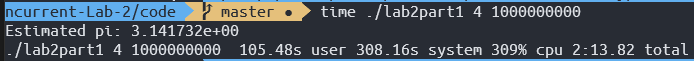
\includegraphics[width=\textwidth]{Figures/part1_4_10e9.PNG}
	\caption{Terminal output of lab2part1.c program using $10^9$ tosses with 4 threads}
	\label{fig:part1_4_10e9}
\end{figure}

\begin{figure}[ht]
	\centering
	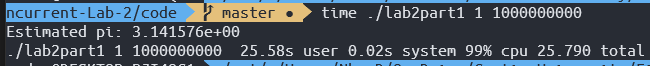
\includegraphics[width=\textwidth]{Figures/part1_1_10e9.PNG}
	\caption{Terminal output of lab2part1.c program using $10^9$ tosses with 1 threads}
	\label{fig:part1_1_10e9}
\end{figure}

The estimated values for $\pi$ was accurate to 3 decimal places. It took 2:13.82s to compute $\pi$ using
$10^9$ samples with 4 threads, and only 25.790s to compute with 1 thread per \cref{fig:part1_4_10e9} 
and \cref{fig:part1_1_10e9} respectively.  % Monte Carlo's extimation of Pi using POSIX's pthreads	

%----------------------------------------------------------------------------------------
%  Trapezoid rule with POSIX's Pthreads
%----------------------------------------------------------------------------------------

\section{Trapezoid rule with POSIX Pthreads}

\subsection{Creating threads using POSIX}

\vspace{0.5cm}
\lstinputlisting[
	style=CStyle,
	firstline=72, % First line of code
	lastline=75, % Lastl ine of code
	caption=Creating POSIX Pthreads (line 72-75 in lab2part2.c), % Caption above the listing
	label=lst:lab2part2a, % Label for referencing this listing
	frame=single, % Frame around the code listing
	showstringspaces=false, % Don't put marks in string spaces
	numbers=left, % Line numbers on left
	numberstyle=\normalsize % Line numbers styling
    ]{../code/lab2part2.c}

%----------------------------------------------------------------------------------------

\subsection{Joining threads using POSIX}

\vspace{0.5cm}
\lstinputlisting[
	style=CStyle,
	firstline=77, % First line of code
	lastline=80, % Lastl ine of code
	caption=Joining POSIX Pthreads (line 77-80 in lab2part2.c), % Caption above the listing
	label=lst:lab2part2b, % Label for referencing this listing
	frame=single, % Frame around the code listing
	showstringspaces=false, % Don't put marks in string spaces
	numbers=left, % Line numbers on left
	numberstyle=\normalsize % Line numbers styling
    ]{../code/lab2part2.c}

%----------------------------------------------------------------------------------------

\subsection{If each thread is allowed to increment the total sum on the fly, does a race condition exist?
If so, how does this affect the final result?}

With syncronisation, a race condition will exist when multiple thread increment the total sum at the same
time. This affects teh final result by making the global total sum to be less than the actual sum due
increments that were unaccounted for because they were done at the same time.

%----------------------------------------------------------------------------------------

\subsection{Mutex based critical section}

\vspace{0.5cm}
\lstinputlisting[
	style=CStyle,
	firstline=120, % First line of code
	lastline=122, % Lastl ine of code
	caption=Mutex based threads synchronisation (line 120-122 in lab2part2.c), % Caption above the listing
	label=lst:lab2part2c, % Label for referencing this listing
	frame=single, % Frame around the code listing
	showstringspaces=false, % Don't put marks in string spaces
	numbers=left, % Line numbers on left
	numberstyle=\normalsize % Line numbers styling
    ]{../code/lab2part2.c}

%----------------------------------------------------------------------------------------

\subsection{Semaphore based critical section}

\vspace{0.5cm}
\lstinputlisting[
	style=CStyle,
	firstline=110, % First line of code
	lastline=112, % Lastl ine of code
	caption=Semaphores based threads synchronisation (line 120-122 in lab2part2.c), % Caption above the listing
	label=lst:lab2part2d, % Label for referencing this listing
	frame=single, % Frame around the code listing
	showstringspaces=false, % Don't put marks in string spaces
	numbers=left, % Line numbers on left
	numberstyle=\normalsize % Line numbers styling
    ]{../code/lab2part2.c}

%----------------------------------------------------------------------------------------

\subsection{Busy-wait based critical section}

\vspace{0.5cm}
\lstinputlisting[
	style=CStyle,
	firstline=115, % First line of code
	lastline=117, % Lastl ine of code
	caption=Busy-wait based threads synchronisation (line 115-117 in lab2part2.c), % Caption above the listing
	label=lst:lab2part2e, % Label for referencing this listing
	frame=single, % Frame around the code listing
	showstringspaces=false, % Don't put marks in string spaces
	numbers=left, % Line numbers on left
	numberstyle=\normalsize % Line numbers styling
    ]{../code/lab2part2.c}

%----------------------------------------------------------------------------------------

\subsection{Results}

The code was compile to compute the trapezoid rule for $a=0$, $b=1$, $n=2^{30}$ for the function $f(x)$.
128 threads were used for each of the three methods (mutex, semaphores, busy-wait) to determine whic method is the fastest.
The function $f(x)$ is hardwired to compute $x^2$, see \cref{lst:lab2part2f}.

\vspace{0.5cm}
\lstinputlisting[
	style=CStyle,
	firstline=151, % First line of code
	lastline=159, % Lastl ine of code
	caption=Hardwired f(x) for trapezoid rule (line 154-159 in lab2part2.c), % Caption above the listing
	label=lst:lab2part2f, % Label for referencing this listing
	frame=single, % Frame around the code listing
	showstringspaces=false, % Don't put marks in string spaces
	numbers=left, % Line numbers on left
	numberstyle=\normalsize % Line numbers styling
    ]{../code/lab2part2.c}

Linux echo was use to pipe in the user input so that it does not vary execution the execution time. Linux's
time command was used to time the different synchronisation methods. The results are shown in 
\cref{fig:part2_128_0,fig:part2_128_1,fig:part2_128_2}.

\begin{figure}[ht]
	\centering
	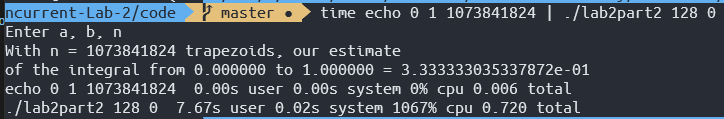
\includegraphics[width=\textwidth]{Figures/part2_128_1.PNG}
	\caption{Terminal output of lab2part2.c program using 128 threads and mutex}
	\label{fig:part2_128_0}
\end{figure}

\begin{figure}[ht]
	\centering
	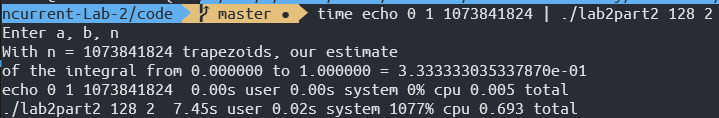
\includegraphics[width=\textwidth]{Figures/part2_128_2.PNG}
	\caption{Terminal output of lab2part2.c program using 128 threads and semaphores}
	\label{fig:part2_128_1}
\end{figure}

\begin{figure}[ht]
	\centering
	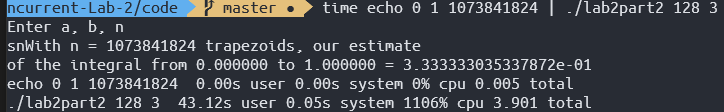
\includegraphics[width=\textwidth]{Figures/part2_128_3.PNG}
	\caption{Terminal output of lab2part2.c program using 128 threads and busy-wait}
	\label{fig:part2_128_2}
\end{figure}

The result shows that semaphores is the fastest, then mutex and then busy-wait in terms of execution time.
Busy wait is the least efficient because it consumes CPU cycles as the threads continously wait. Busy-wait
enfores the order of access to the critical section, and waits for the system to schedule on the thread
rank matching the flag variable to allow be allowed through - if it schedules on the wrong thread (a thread
that is busy-waiting), it wastes CPU cycles in the checking of the while condition until it deschedules and 
eventually until it picks the correct thread.

Mutex is middle between the three, only slower than semaphores by 40ms. The order the threads execute
the critical section is random, which does not guarentee that locks are given in the order they are called. % Trapezoid rule with POSIX's Pthreads

\end{document}
